\chapter{Les Progiciels de Gestion Internes}

\section{Introduction}
Le but de ce chapitre est de présenter globalement le progiciel de gestion interne aussi appeler \acs{ERP}.\\

Dans un premier temps, nous définirons le concept d'\acs{ERP} et son évolution dans le temps.\\

Par la suite, nous aborderons les avantages liés a l'intégration d'un tel système dans les deux aspects administratif et opérationnel ainsi que ses inconvénients.\\

Nous finirons avec les multiples fonctionnalités de l'\acs{ERP}.\\

\section{Définition}
L'acronyme \acs{ERP} signifie Entreprise Resource Planning, et sa similitude en français est Progiciel de Gestion Intégré abrévié \acs{PGI}.\\

Contrairement au \acs{MRP} (Manufacturing Resource Planning) qui se contente de la planification des besoins, l'\acs{ERP} est un logiciel qui permet la gestion de tous les sous-systèmes de l'entreprise et la coordination de ces sous-systèmes.\\

Pour y parvenir l’\acs{ERP} intègre toutes les fonctions utiles de l'entreprise sous forme de modules qui partagent une seule base de données, ce qui permet l'échange d'informations entre modules, dans ce cas, on parle de moteurs de workflow.\\

\section{Historique}
Joseph Orlicky a été à l'origine de la création de l'\acs{ERP}. Il a créé l'acronyme de \acs{MRP} dans les années 1960, qui est l'ancêtre de la planification de la demande matérielle d'\acs{ERP}. \acs{MRP} répond principalement aux besoins de planification de l'entreprise.\\

Le concept d'\acs{ERP} tel que nous le connaissons est apparu pour la première fois dans les années 1990, mais avec l'avènement d'Internet, il n'a commencé à se développer que dans les années 2000. L'utilisation de l'\acs{ERP} s'est généralisée et a évolué vers l'\acs{ERP} tel que nous le connaissons aujourd'hui.

\section{Avantages liés à l’intégration d’un \acs{ERP}}
Plusieurs études ont démontré les bénéfices de la mise en place d'un \acs{ERP}, dont l'une a été menée par Aberdeen Group, qui a quantifié et publié les résultats suivants :\\

\begin{itemize}
    \item Réduction des coûts d’opérations de 22\%
    \item Réduction des coûts d’administration de 20\%
    \item Réduction d’inventaires de 17\%
    \item Amélioration du temps de livraison de 19\%
    \item Amélioration du respect des délais et des budgets de 17\%\\
\end{itemize}

Même les entreprises en difficulté ont réalisé des avantages en intégrant l'\acs{ERP}, et le résultat est :\\

\begin{itemize}
    \item Réduction des coûts d’opérations de 7\%
    \item Réduction des coûts d’administration de 4\%
    \item Réduction d’inventaires de 9\%
    \item Amélioration du temps de livraison de 11\%
    \item Amélioration du respect des délais et des budgets de 6\%\\
\end{itemize}

Comme le souligne la recherche, les avantages en pourcentage ne semblent pas impressionnants, mais pour chaque million de dollars dépensé en coûts d'exploitation, des économies de 70 000 \$ sont réalisées.\\

En effet, on peut constater l'amélioration de la productivité et de la maturité des entreprises. Pour y parvenir, l'\acs{ERP} a été amélioré sous plusieurs aspects : \\

\subsection{Aspect administratif}
En consolidant tous les systèmes de l'entreprise en une seule application, l'installation de l'\acs{ERP} peut réduire les coûts d'exploitation et de maintenance, et parce que l'\acs{ERP} a une architecture modulaire, il fournit une infrastructure qui peut assurer la flexibilité à l'avenir lorsque des changements se produisent.\\

Une seule application, donc une seule base de données, cette seule base de données permet de gagner du temps. Réduire la quantité d'informations inutiles et évitez les saisies multiples. L'installation de l'\acs{ERP} résout le problème des informations incohérentes et fiabilise les données enregistrées.\\

De plus les activités manuelles de traitement, de comparaison et de recherche réalisée par les employés dans le cadre de l'interface des différents services sont évitées. Cela conduit à un gain de croissance, de temps et de productivité administrative.\\ 

\subsection{Aspect opérationnel}
L'utilisation de l'\acs{ERP} permet d'éliminer les risques opérationnels et les risques de pertes liés aux erreurs humaines ou aux défaillances du contrôle interne, et les fraudes qui peuvent être provoquées par les défaillances du système d'information existant. Les coûts supplémentaires inutiles dus aux dysfonctionnements sont réduits et une pertinence des informations partagées est gagnée.\\

L'\acs{ERP} permet également un suivi au niveau de l'achat jusqu'à la vente. En effet, dès la création de la commande, des données telles que la marge et le crédit sont générés automatiquement de manière dynamique pour réaliser l'intégration financière. Avec cette fonction, l'\acs{ERP} aide les managers dans le processus de planification et de prise de décision, et leur permet d'améliorer la gestion des ressources, ainsi améliorer la prise de décision opérationnelle.\\

De plus, les services de finances bénéficient de la centralisation. Cette centralisation permet de réunir les taches dans un seul endroit, ce qui a son tour permet l'amélioration de la productivité en réduisant le nombre d'employés nécessaires qui travaille sur la même tâche, cela permet d'augmenter les économies d’échelles notamment en matière de facturation.\\

\section{Inconvénients\cite{cxp-2017}}
L'\acs{ERP} offre des avantages importants, mais une telle solution doit présenter certains inconvénients.\\

Les projets \acs{ERP} entraînent généralement des coûts lors de la configuration et de la maintenance. De plus, la complexité des programmes utilisés nécessite l'utilisation et la maintenance de serveurs puissants. Cela signifie que comme le montre l'étude CXP 2017, les coûts sont souvent dépassés.\\

\begin{figure}[H]
    \centering
    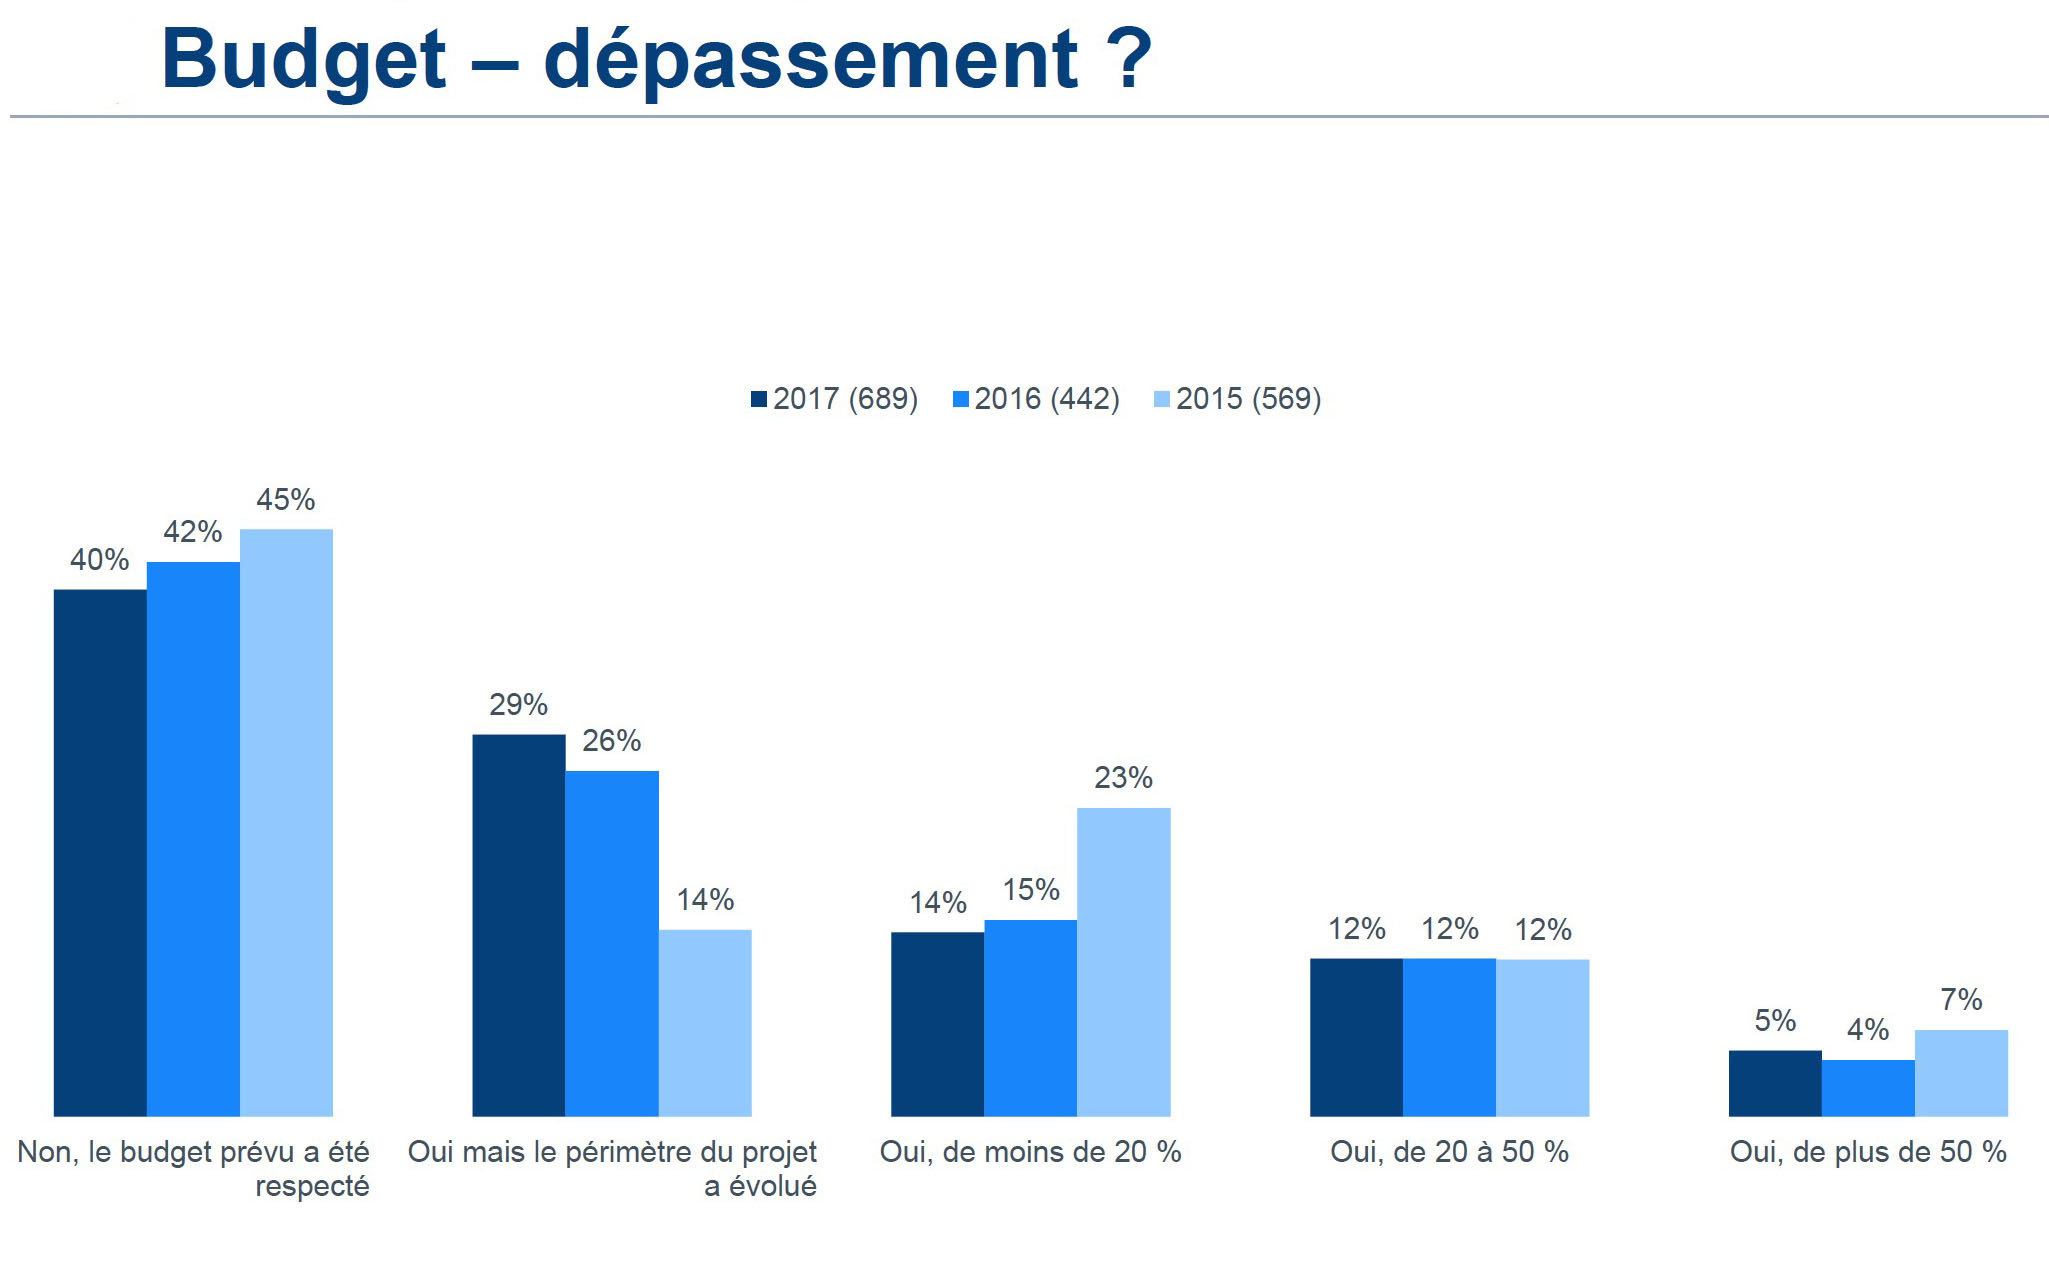
\includegraphics[scale=0.4]{ERP/graph-depassement-budget.jpg}
    \caption{Taux du dépassement de budget lors de l’implémentation d’un ERP}
\end{figure} 

On peut constater qu’en 2017 plus de 60\% des entreprises qui ont implémenté un \acs{ERP} ont dépassé le budget prévu, 58\% en 2016 et 55\% en 2015.\\

En plus du coût, comme le montre l'étude 2010 du rapport ERP du cabinet de conseil Panorama Consulting\cite{panorama-consulting}, un projet d'une telle envergure peut nécessiter plus de temps et de ressources que prévu.\\

\begin{figure}[H]
    \centering
    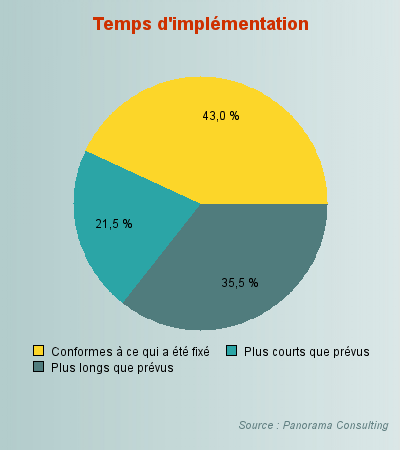
\includegraphics[scale=0.65]{ERP/graph-taux-implementation.png}
    \caption{Taux des dépassements des délais lors de l’implémentation d’un ERP}
\end{figure} 

Cette étude montre que plus de 35,5\% des entreprises ont mis en place un \acs{ERP} et constatent que le délai de mise en place a dépassé le délai autorisé. Il faut également noter que la durée moyenne de mise en place de l'\acs{ERP} est de 18 ou 4 mois, d'un éditeur à l'autre.\\

\section{Fonctionnalités}
L'ERP gère et organise automatiquement et dynamiquement les informations des différents services de l'entreprise, de l'approvisionnement des ressources aux ventes en passant par la production, ces fonctions sont nombreuses. Les modules les plus couramment utilisés sont :\\

\begin{itemize}
    \item Gestion de production
    \item Gestion de stock et d’inventaire
    \item Gestion des ressources humaines 
    \item Gestion de la chaine logistique
    \item Gestion de projet
    \item Gestion comptabilité
    \item Gestion commerciale
    \item Gestion d’achats
    \item CRM : Gestion des relations clients\\
\end{itemize}

Chaque module couvre ses propres fonctions, et le tableau suivant résume certains des modules et les fonctions qu'ils fournissent.

\begin{table}[H]
    \begin{center}
        
        \begin{tabular}{|F{4cm}|R{10cm}|}
            \hline
            \textbf{Modules}  & \makecell[c]{\textbf{Fonctionnalités}} \\
            \hline
            Achats
            &
            Gestion de toutes les transactions comptables, telle que les bons de commande pour l’approvisionnement. Etc.\\
            
            \hline
            Chaine logistique
            &
            Gestion des ressources utilisées pour le pilotage de la chained’approvisionnement et de livraison.\\
            
            \hline
            Stock
            &
            Gestion des mouvements du stock, état du stock, entreposage.\\
            
            \hline
            Production
            &
            La gestion de la production, permet de réguler l’offre et les besoins en
            ressources par apport à la demande, impliquent la planification des ordres
            de fabrication et le contrôle de qualité.\\
            
            \hline
            Gestion de projet
            &
            Gestion de l’ensemble des projets de l’entreprise, de ces tâches et de ces plannings.\\
            
            \hline
            Ressources humaines
            &
            Gestion des ressources humaines et l’organisation de la rémunération des employés ainsi que des plannings de travail de ceux-ci.\\
            
            
            \hline
            Comptabilité
            &
            Gestion des obligations comptable auxquelles l’entreprise est soumise et suivie en temps réel de la santé financière de celle-ci, ainsi que de la gestion de facturation et des multidevises.\\
            
            \hline
            Commerciale
            &
            Gestion de l’aspect commerciale de l’entreprise, permet la gestion de l’ensemble des commandes clients et de leur facturation, permet aussi la réalisation de devis rapide et précise.\\
            
            \hline
            CRM
            &
            Gestion des relations clients, permet de réaliser de meilleurs suivis de
            l’environnement : clients, fournisseurs, prospects. etc.\\
            
            
            \hline
        \end{tabular}	
        \caption{Les Modules d'un ERP et leurs fonctionnalités}
    \end{center}
\end{table}

\section{Conclusion}
Après avoir défini lors de la première partie le concept d’entreprise, l’environnement et les contraintes auxquelles elle fait face. L’obligation de dégager un bénéfice est vitale, mais un certain nombre de points complexifient leurs systèmes d’information et freine la croissance économique de celle-ci, ces mêmes points qui rendent le recours à une technologie de l’information telle que l’ERP presque obligatoire.\\

Dans le deuxième point nous avons étudié l’ERP qui est au cœur du système d’information et qui permet la gestion de tous les services de l’entreprise. Ainsi que les avantages et les inconvénients à recourir à un tel outil.\\

Ensuite nous allons approfondir la recherche et étudier lors du deuxième chapitre, la gestion de stocks et d’approvisionnement.


\newpage

\leftskip=0cm
\renewcommand{\bibname}{Référence bibliographique et webographique du chapitre 1}
\bibliographystyle{ieeetr}	
\bibliography{ERP/erp}